\documentclass[12pt, a4paper, simple]{eskdtext}

\usepackage{hyperref}
\usepackage{env}
\usepackage{_sty/gpi_lst}
\usepackage{_sty/gpi_toc}
\usepackage{_sty/gpi_t}
\usepackage{_sty/gpi_p}
\usepackage{_sty/gpi_u}

% Код
\ESKDletter{}{К}{Р}
\def \gpiDocTypeNum {81}
\def \gpiDocVer {00}
\def \gpiCode {\ESKDtheLetterI\ESKDtheLetterII\ESKDtheLetterIII.\gpiStudentGroupName\gpiStudentGroupNum.\gpiStudentCard-0\gpiDocNum~\gpiDocTypeNum~\gpiDocVer}

\def \gpiDocTopic {ПОЯСНИТЕЛЬНАЯ ЗАПИСКА}

% Графа 1 (наименование изделия/документа)
\ESKDcolumnI {\ESKDfontIII \gpiTopic \\ \gpiDocTopic}

% Графа 2 (обозначение документа)
\ESKDsignature {\gpiCode}

% Графа 9 (наименование или различительный индекс предприятия) задает команда
\ESKDcolumnIX {\gpiDepartment}

% Графа 11 (фамилии лиц, подписывающих документ) задают команды
\ESKDcolumnXIfI {\gpiStudentSurname}
\ESKDcolumnXIfII {\gpiTeacherSurname}
\ESKDcolumnXIfV {\gpiTeacherSurname}

\begin{document}
    \begin{ESKDtitlePage}
    \begin{center}
        \gpiMinEdu \\
        \gpiEdu \\
        \gpiKaf \\
    \end{center}

    \vfill

    \begin{flushright}
        \begin{minipage}[t]{.45\textwidth}
            <<К защите допускаю>> \\
            \gpiHeadDepartmentInfo \\
            \underline{\hspace{3cm}} \gpiHeadDepartmentName~\gpiHeadDepartmentSurname \\
            \PageTitleDateField
        \end{minipage}
    \end{flushright}

    \vfill

    \begin{center}
        \gpiTopic \\
    \end{center}

    \vfill

    \begin{center}
        \textbf{\gpiDocTopic} \\
        ПО ДИСЦИПЛИНЕ \gpiDiscipline \\
    \end{center}

    \vfill

    \begin{center}
        \gpiCode \\
        Листов \pageref{LastPage} \\
    \end{center}

    \vfill

    \begin{flushright}
        \begin{minipage}[t]{.49\textwidth}
            \begin{minipage}[t]{.75\textwidth}
                \begin{flushright}
                    Руководитель

                    \hspace{0pt}

                    Выполнил

                    \hspace{0pt}

                    Консультанты:

                    по ЕСПД

                    Рецензент
                \end{flushright}
            \end{minipage}
        \end{minipage}
        \begin{minipage}[t]{.49\textwidth}
            \begin{flushright}
                \begin{minipage}[t]{.75\textwidth}
                    \gpiTeacherName~\gpiTeacherSurname

                    \hspace{0pt}

                    \gpiStudentName~\gpiStudentSurname

                    \hspace{0pt}

                    \hspace{0pt}

                    \gpiTeacherName~\gpiTeacherSurname

                    \gpiReviewerName~\gpiReviewerSurname
                \end{minipage}
            \end{flushright}
            
        \end{minipage}
    \end{flushright}

    \vfill

    \begin{center}
        \ESKDtheYear
    \end{center}
\end{ESKDtitlePage}


    \ESKDthisStyle{empty}
    лист с заданием
    \newpage
    \ESKDthisStyle{formII}

    % Содержание
    \tableofcontents                                
    \paragraph{ПРИЛОЖЕНИЕ А. СХЕМА ПРОГРАММЫ}
    \paragraph{ПРИЛОЖЕНИЕ Б. ТЕКСТ ПРОГРАММЫ}
    \newpage

    %
    \newpage
    \addcontentsline{toc}{section}{ВВЕДЕНИЕ}
    \section*{ВВЕДЕНИЕ}

    Цель курсовой работы по дисциплине <<Совремменные платформы программирования>> - детальное проектирование и программная реализация сетевой игры.

    Клиенская часть написана на языке программирования Java Script, с использованием фреймворка ReactJS,
    с использованием объектно-ориентированного программирования.
    Серверная часть написана на языке программирования Node Java Script.

    Используя объектно-ориентированное проектирование позволяет обходить ряд сложных проблем в программировании,
    сводя необходимую модификацию программы к её расширению и дополнению.
    Систематическое применение объектно-ориентированного подхода позволяет разрабатывать достаточно хорошо структурированные,
    надежные в эксплуатации, просто модифицируемые программные системы.
    Элементы объектно-ориентированного программирования получили своё развитие, и в настоящее время ООП принадлежит к числу ведущих технологий программирования.

    \newpage

    %
    \section{АНАЛИЗ ПОСТАВКИ ЗАДАЧИ}
    \subsection{Перечень функций}

    Достижение цели курсовой работы предполагает необходимость создания веб- или мобильное приложение (ОС Android/iOS) со следующим функционалом:
    
    \begin{enumerate}
        \item[1.] Предусмотреть возможность игры с ИИ.
        \item[2.] Разработать фиксированный набор карт для игры (от 30 и более).
        \item[3.] Сохранение статистики матчей (опционально - сохранение на удаленном сервере).
        \item[4.] Поддержка сетевого матча один-на-один.
        \item[5.] Минимальный пользовательский интерфейс и графическое оформление карт.
    \end{enumerate}
    
    \subsection{Требования пользователей}

    Пользовательские требования - описание на естественном языке (плюс поясняющие диаграммы) функций, выполняемых системой, и ограничений, накладываемых на неё.

    Ответственный: Системный аналитик

    Эти требования должны определять только внешнее поведение системы, избегая по возможности определения структурных характеристик системы.
    Пользовательские требования должны быть написаны естественным языком с использованием простых таблиц, а также наглядных и понятных диаграмм.

    \textbf{Обязательные} требования игрока к игре:

    \begin{enumerate}
        \item [1.] Разработать фиксированный набор карт для игры (от 30 и более).
        \item [2.] Минимальный пользовательский интерфейс и графическое оформление карт.
    \end{enumerate}

    \textbf{Желательные} требования к игре:

    \begin{enumerate}
        \item [1.] Предусмотреть возможность игры с ИИ.
        \item [2.] Сохранение статистики матчей (опционально - сохранение на удаленном сервере).
        \item [3.] Поддержка сетевого матча один-на-один.
    \end{enumerate}

    \newpage
    \subsection{Описание предметной области}

    \textbf{Игрок} - человек или машина, который/которая играет в данную игру.
    В данной игре будут два игрока: мы и игрок противник.

    \textbf{Карты} - графический элемент игры, в виде прямоугольника с характеристиками.
    Карт в игре в количестве 30 штук. 30 штук как и у нас, так и у противника.
    Карты имеют фракции: мечник, лучник, тяжелая альтилерия; который сдавятся в определеное поле боя.
    
    \textbf{Мечник} - категория карты, которая имеет малый урон и сражается с мечниками противника.

    \textbf{Лучник} - категория карты, которая имеет малый урон и сражается с лучниками противника.

    \textbf{Тяжелая альтилерия} - катерия карты, которая имеет высокий урон и сражается с тяжелой альтилерией противника.

    \textbf{Поле боя} - игровое поле, которое разбито на 6 частей, из которых три части противника и три части наши.
    
    Поле боя содержит:

    \begin{enumerate}
        \item [1.] Тяжелую альтилерию противника.
        \item [2.] Лучников противника.
        \item [3.] Мечников противника.
        \item [4.] Своих мечников.
        \item [5.] Своих лучников.
        \item [6.] Свою тяжелую альтилерию.
    \end{enumerate}

    \textbf{ПАС} - действие, после объявления которого мы объявляем о прекращении бойни и пропускаем ход, в тоже время противнику дается последний выбор карты,
    после чего подсчитывается игровой счёт. В течении игры можна два раза нажать на кнопку <<ПАС>>.
    После подсчёта первого <<ПАС>> карты с поля боя идут на кладбище. Набираются карты до десяти.
    Происходит игра. После подсчёта второго <<ПАС>> сравниваются победы и объявляется победитель.

    \newpage
    \subsection{Варианты использования программы в виде диаграмм прецедентов (use case diagram)}

    Варианты использования программы изображены на рис.~\ref{fig:game__use_case_diagram}.

    \begin{figure}[!h]
        \centering
        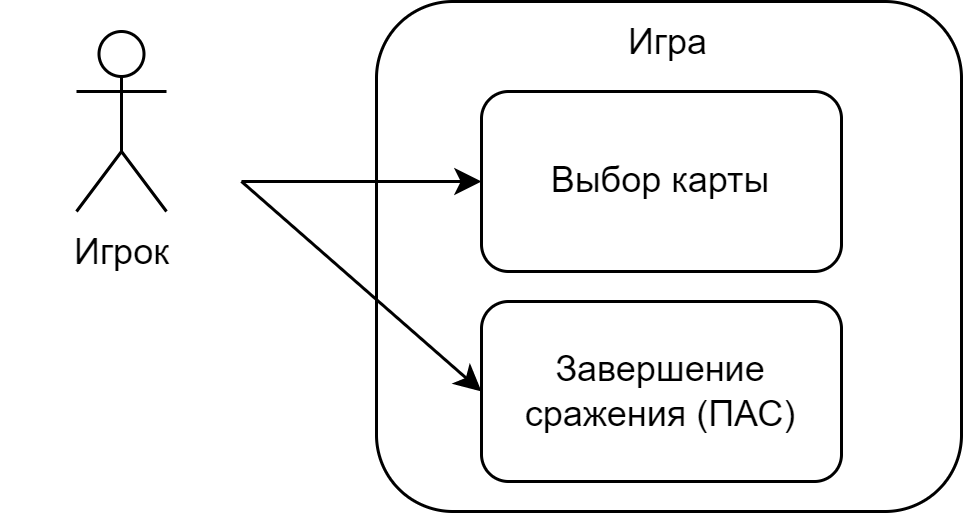
\includegraphics[]
            {../sources/game_architecture/build/game__use_case_diagram.png}
        \caption{Первичное описание прецедентов}
        \label{fig:game__use_case_diagram}
    \end{figure}

    \paragraph{}\hspace{0pt}

    \textbf{\underline{Прецендент №1 <<Выбор карты>>}}

    \textbf{Назначение}: из своей колоды карт выбираем карту, которую ходим выставить на поле.

    \textbf{Исполнители}: игрок.

    \textbf{Предусловие}: есть карта/карты, которую/которые можно выбрать.

    \textbf{Основной поток событий}: игрок выберет карту и карты попадет на поле (мечника, лучника, тяжелой альтилерии),
    иначе АПС.

    \textbf{Альтернативный поток событий}: если у игрока не будет карт, то игрок пропускает ход;
    если игрок не выбирает карту, то по истечению времени карта выбирается автоматически.

    \paragraph{}\hspace{0pt}

    \textbf{\underline{Прецендент №2 <<Завершения сражения (ПАС)>>}}

    \textbf{Назначение}: завершить бой и узнать результат бойни.

    \textbf{Исполнители}: игрок.

    \textbf{Предусловие}: есть карты на поле.

    \textbf{Основной поток событий}: мы пропускаем ход, а противник выбирает последнюю карту, после чего проиходит подчёт сил, иначе АПС.

    \textbf{Альтернативный поток событий}: игрок может продолжать выставлять карты на поле.

    \newpage
    % \subsection{Первичное описание объектов и классов, прецедентов системы}
    \subsection{Первичное описание объектов и классов}

    Первичное описание класса игры изображено на рис.~\ref{fig:game__first_class_diagram}.

    \begin{figure}[!h]
        \centering
        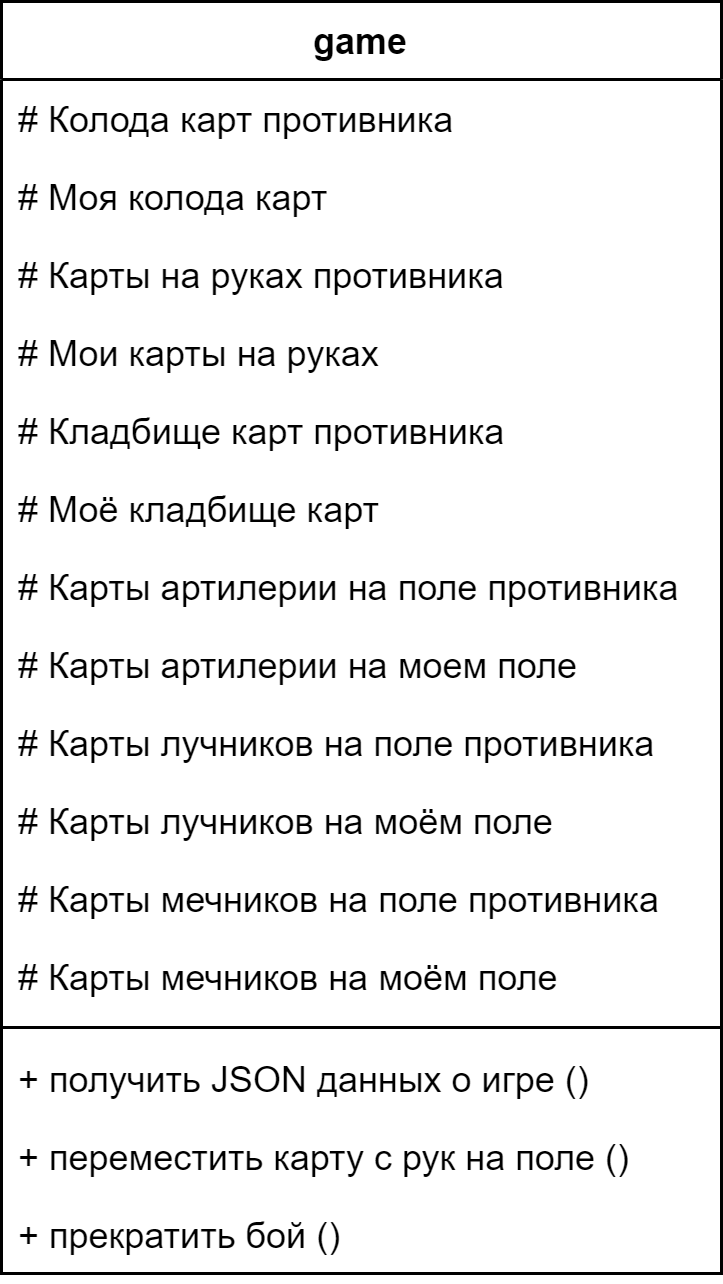
\includegraphics[]
            {../sources/game_architecture/build/game__first_class_diagram.png}
        \caption{Первичное описание класса игры}
        \label{fig:game__first_class_diagram}
    \end{figure}

    Игра - класс содержащий логику игры.

    \begin{itemize}
        \item Колода карт противника и моя колода карт - начальный стак карточек,
        из которых в начале игры берется 10 рандомных карт.
        \item Карты на руках противника и мои карты на руках - карты, которые держим в руках,
        не могут превышать 10 штук. При количестве 0 штук - игрок пропускает ход.
        \item Кладбище карт противника и моё кладбище карт - карты которые ушли в отбой после первого сражения,
        так как игрок сделал ПАС и были подсчитаны результаты боя.
        \item Карты артилерии на поле противника и карты артилерии на моём поле - карты,
        которые выставлены на поле артилерии.
        Могут отсутствовать (0 штук).
        \item Карты лучников на поле противника и карты лучников на моём поле - карты,
        которые выставлены на поле лучников.
        Могут отсутствовать (0 штук).
        \item Карты мечников на поле противника и карты мечников на моём поле - карты,
        которые выставлены на поле мечника.
        Могут отсутствовать (0 штук).
    \end{itemize}

    % \subsection{Первоначаьное описание отношений между классами}

    \newpage
    \subsection{Диаграмма состояний (statechart diagram) для прецендентов}

    Диаграмма состояний для игры изображена на рис.~\ref{fig:game__statechart_diagram}.

    \begin{figure}[!h]
        \centering
        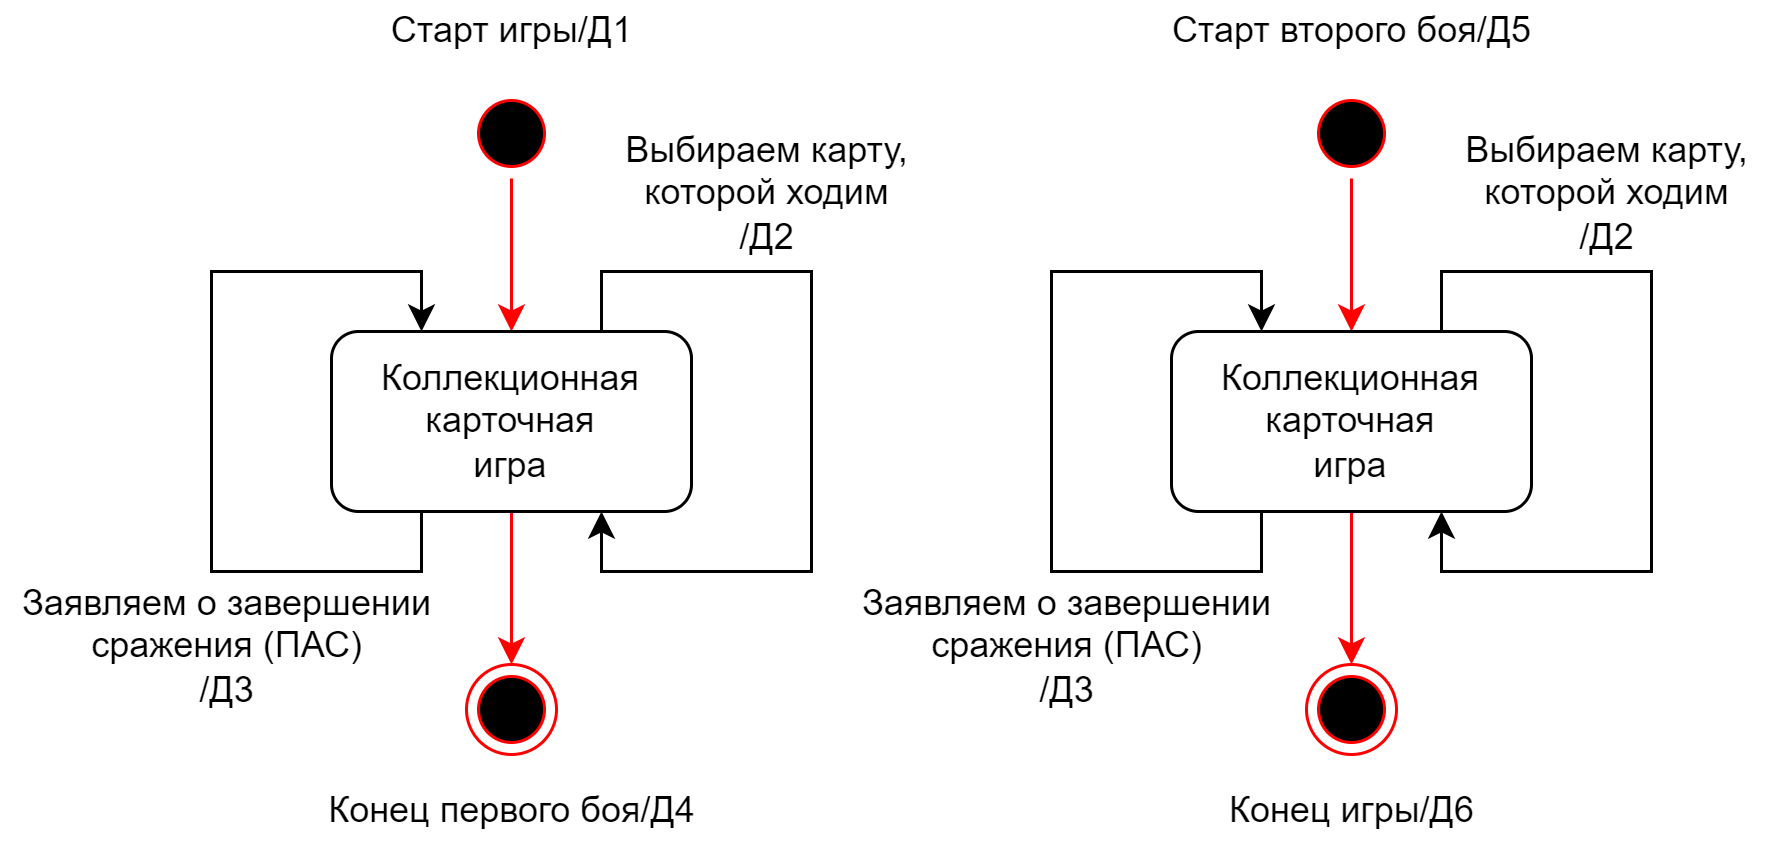
\includegraphics[]
            {../sources/game_architecture/build/game__statechart_diagram.png}
        \caption{Диаграмма состояний игры}
        \label{fig:game__statechart_diagram}
    \end{figure}

    \begin{itemize}
        \item Д1 - Начало игры (быбрали режим: играть с ИИ или играть с другим игроком по сети)
        \item Д2 - Выбираем карту из колоды, которой будет ходить (мечника, лучника, артилерию).
        \item Д3 - Заявляем о завершении боя: мы пропускаем ход, противник кладет последнюю карту, боя заканчивается.
        \item Д4 - Завершение первого боя и подсчёт сил. Старт второго боя
        \item Д5 - Страт второго боя.
        \item Д6 - Завершение второго боя и подсчёт сил. Сравниваются два боя. Объявляется победитель. Завершается игра.
    \end{itemize}

    %
    \newpage
    \section{ПРОЕКТИРОВАНИЕ СТРУКТУРЫ ПРИЛОЖЕНИЯ}

    % \subsection{Диаграммы классов предметной области}
    
    \subsection{Графический интерфейс приложения}
    
    \begin{figure}[!h]
        \centering
        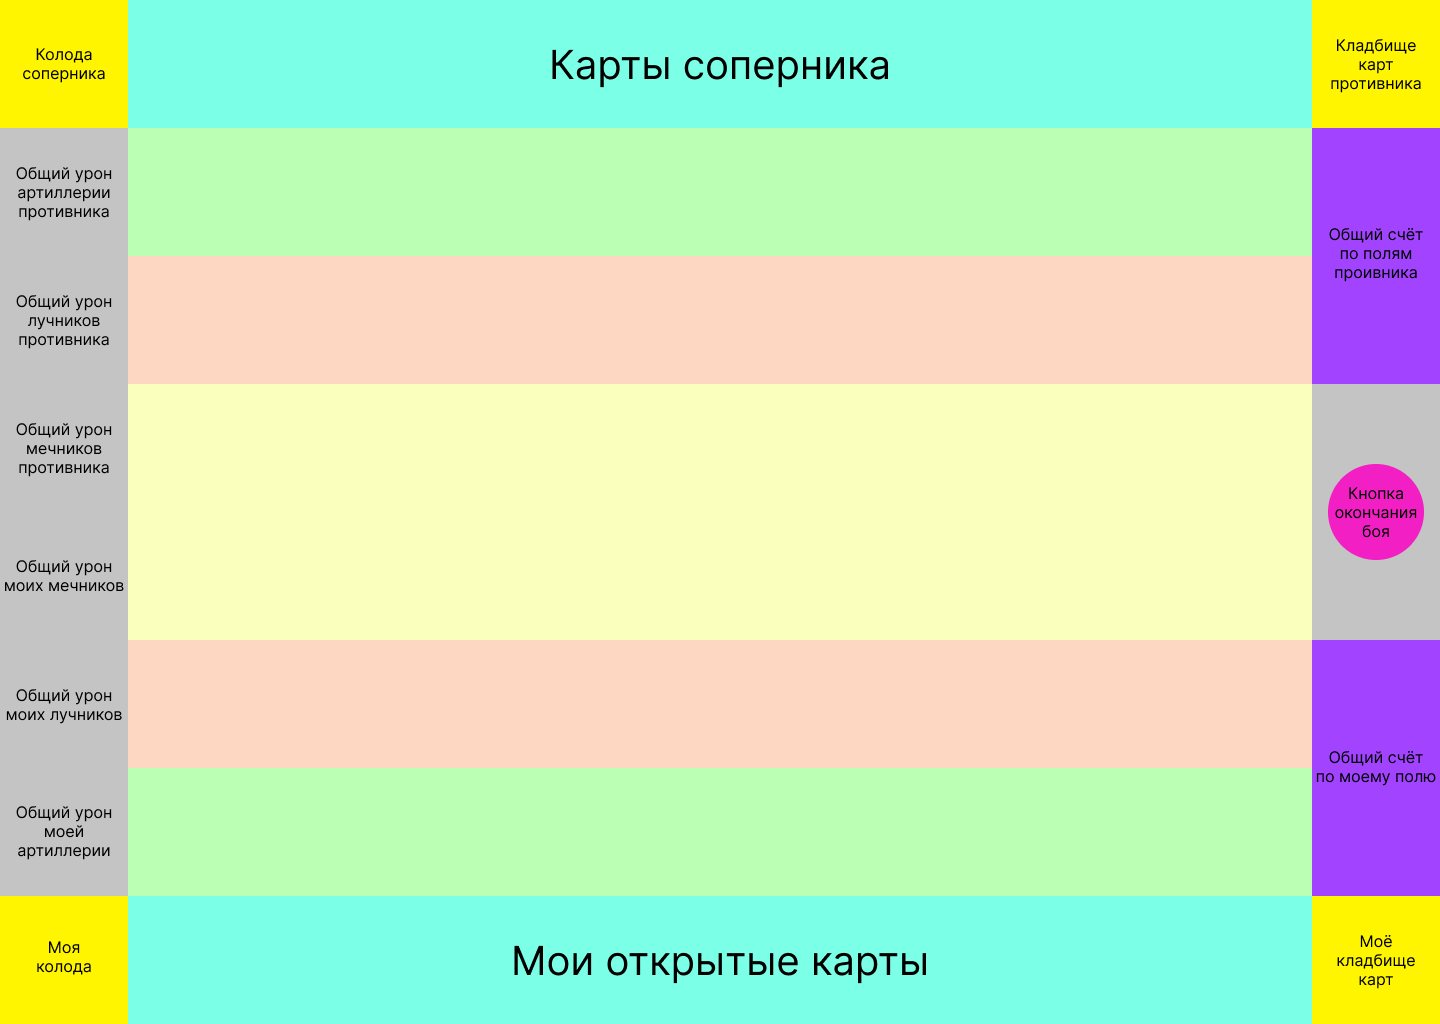
\includegraphics[width=12cm]
            {../sources/game_ux/build/game_ux.png}
        \caption{Макет интерфейса (UX)}
    \end{figure}

    \begin{figure}[!h]
        \centering
        
\includegraphics[width=12cm]
            {../sources/game_ux/build/game_ui.png}
        \caption{Дизайн интерфейса (UI)}
    \end{figure}

    \begin{figure}[p!h]
        \centering
        \begin{minipage}{0.24\textwidth}
            \centering
            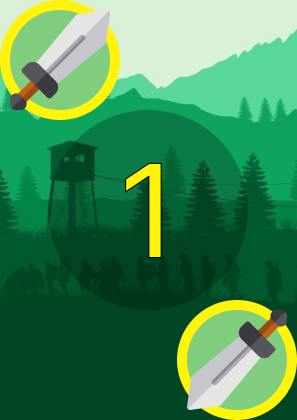
\includegraphics[height=6cm]
                {../sources/game_cards/build/swordsman_card_1.png}
            \caption{Урон 1 мечником}
            \label{fig:swordsman_card_1}
        \end{minipage}
        \begin{minipage}{0.24\textwidth}
            \centering
            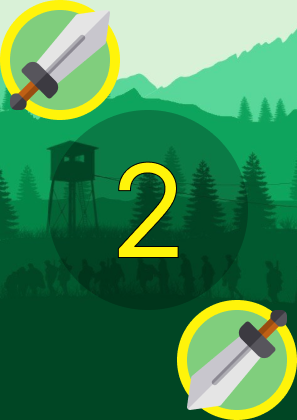
\includegraphics[height=6cm]
                {../sources/game_cards/build/swordsman_card_2.png}
            \caption{Урон 2 мечником}
            \label{fig:swordsman_card_2}
        \end{minipage}
        \begin{minipage}{0.24\textwidth}
            \centering
            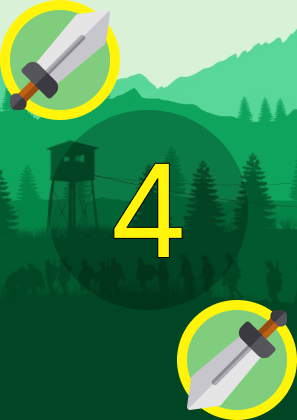
\includegraphics[height=6cm]
                {../sources/game_cards/build/swordsman_card_4.png}
            \caption{Урон 4 мечником}
            \label{fig:swordsman_card_4}
        \end{minipage}
        \begin{minipage}{0.24\textwidth}
            \centering
            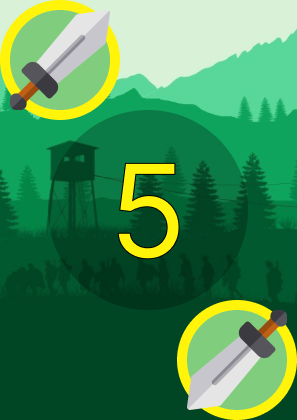
\includegraphics[height=6cm]
                {../sources/game_cards/build/swordsman_card_5.png}
            \caption{Урон 5 мечником}
            \label{fig:swordsman_card_5}
        \end{minipage}
    \end{figure}

    \begin{figure}[p!h]
        \centering
        \begin{minipage}{0.24\textwidth}
            \centering
            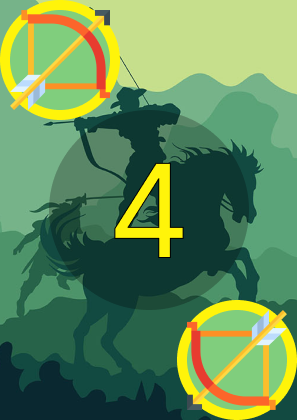
\includegraphics[height=6cm]
                {../sources/game_cards/build/archer_card_4.png}
            \caption{Урон 1 лучником}
            \label{fig:artillery_card_1}
        \end{minipage}
        \begin{minipage}{0.24\textwidth}
            \centering
            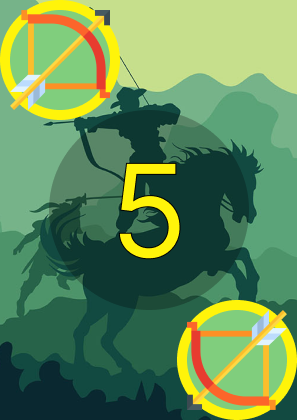
\includegraphics[height=6cm]
                {../sources/game_cards/build/archer_card_5.png}
            \caption{Урон 5 лучником}
            \label{fig:artillery_card_5}
        \end{minipage}
        \begin{minipage}{0.24\textwidth}
            \centering
            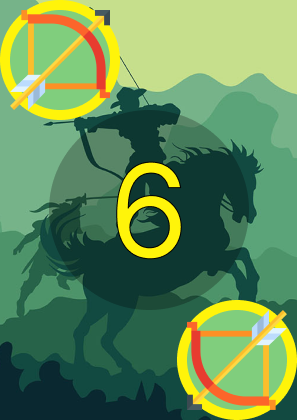
\includegraphics[height=6cm]
                {../sources/game_cards/build/archer_card_6.png}
            \caption{Урон 6 лучником}
            \label{fig:artillery_card_6}
        \end{minipage}
    \end{figure}

    \begin{figure}[p!h]
        \centering
        \begin{minipage}{0.24\textwidth}
            \centering
            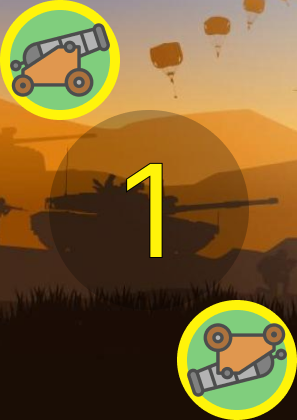
\includegraphics[height=6cm]
                {../sources/game_cards/build/artillery_card_1.png}
            \caption{Урон 1 артилерией}
            \label{fig:artillery_card_1}
        \end{minipage}
        \begin{minipage}{0.24\textwidth}
            \centering
            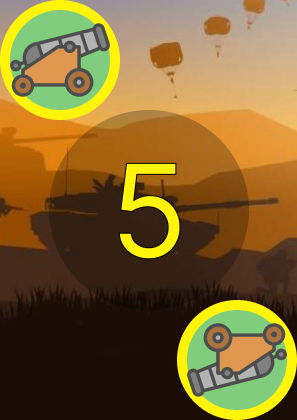
\includegraphics[height=6cm]
                {../sources/game_cards/build/artillery_card_5.png}
            \caption{Урон 5 артилерией}
            \label{fig:artillery_card_5}
        \end{minipage}
        \begin{minipage}{0.24\textwidth}
            \centering
            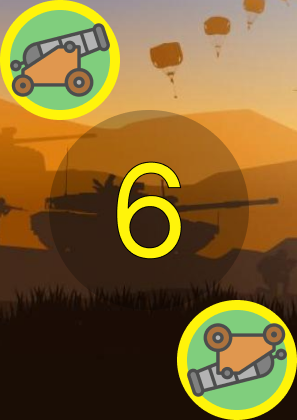
\includegraphics[height=6cm]
                {../sources/game_cards/build/artillery_card_6.png}
            \caption{Урон 6 артилерией}
            \label{fig:artillery_card_6}
        \end{minipage}
        \begin{minipage}{0.24\textwidth}
            \centering
            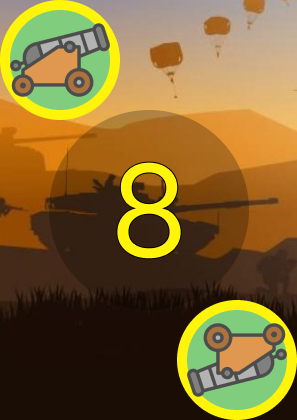
\includegraphics[height=6cm]
                {../sources/game_cards/build/artillery_card_8.png}
            \caption{Урон 8 артилерией}
            \label{fig:artillery_card_8}
        \end{minipage}
    \end{figure}

    % \subsection{Общая диаграмма с учётом каркаса}

    % \subsection{Диаграмма последовательностей (sequence diagram)}
    
    \newpage
    \subsection{Диаграмма видов деятельности (activity diagram)}

    \begin{figure}[!h]
        \centering
        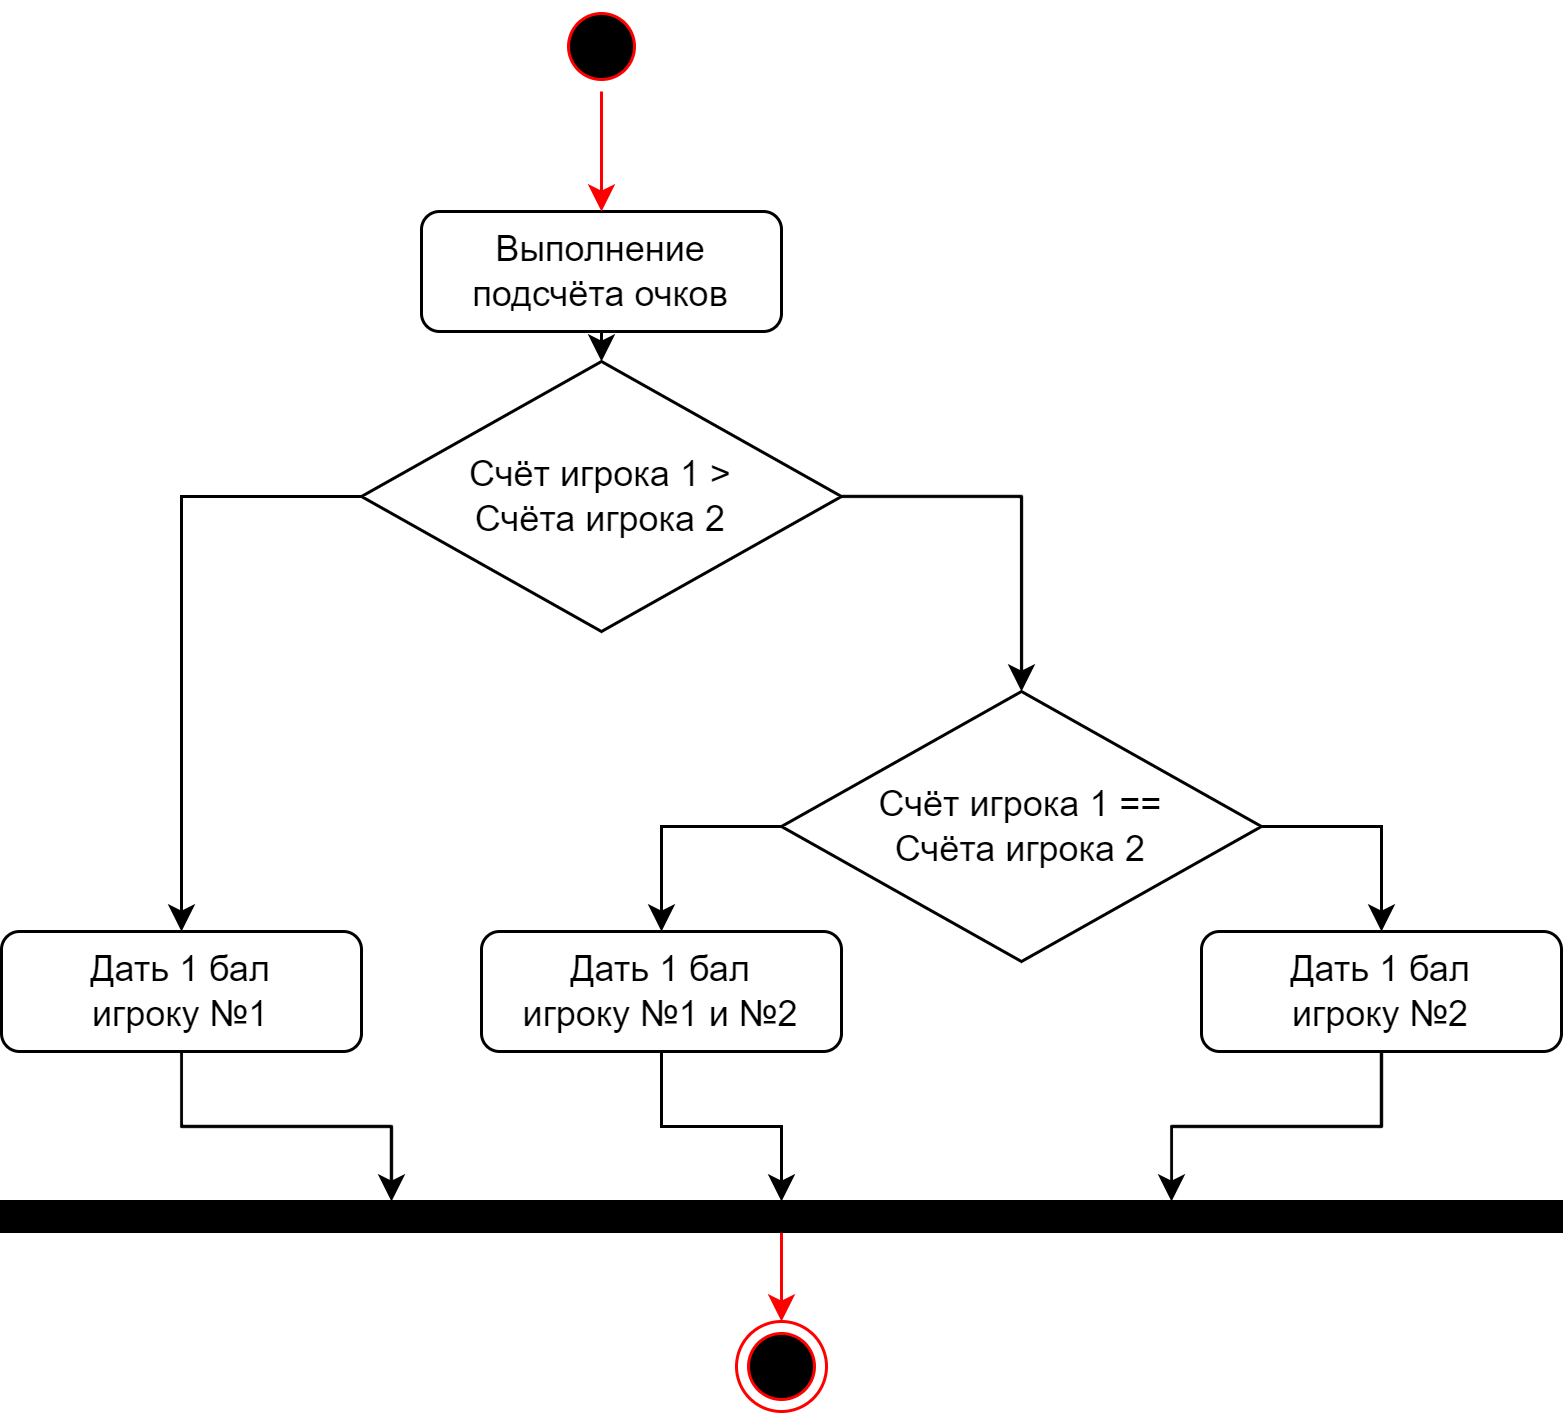
\includegraphics[]
            {../sources/game_architecture/build/game__activity_diagram.png}
        \caption{Деаграмма вида деятельности счётчика балов}
    \end{figure}

    \newpage
    
    %
    \section{РАЗРАБОТКА АЛГОРИТМОВ ФУНКЦИОНИРОВАНИЯ И СТРУКТУР ДАННЫХ}
    \newpage
    
    %
    \section{РЕАЛИЗАЦИЯ ПРИЛОЖЕНИЯ И РЕЗУЛЬТАТЫ ИСПЫТАНИЙ}
    \subsection{Диаграмма компонентов (component diagram)}

    Диаграмма компонентов изображена на рис.~\ref{fig:game__component_diagram}.

    \begin{figure}[!h]
        \centering
        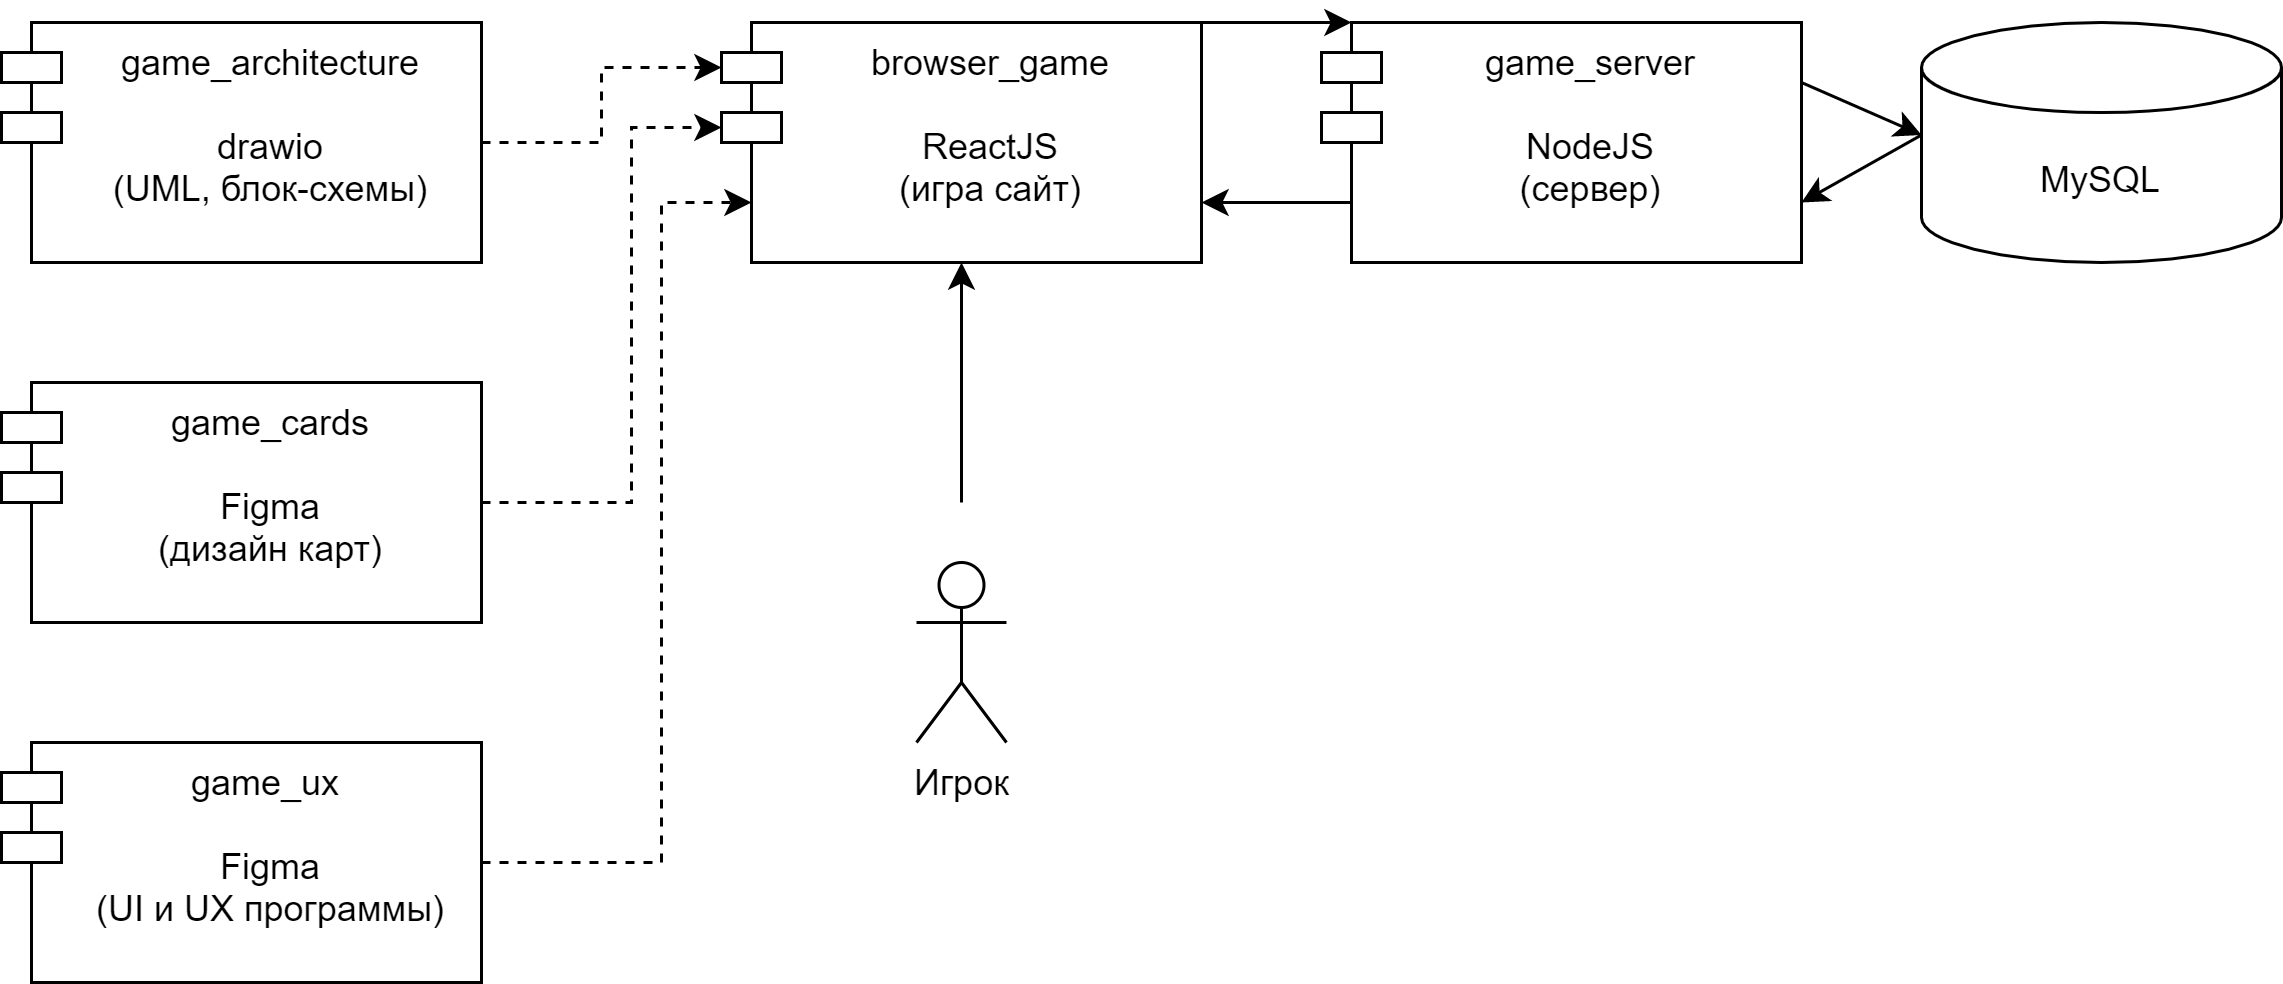
\includegraphics[width=16cm]
            {../sources/game_architecture/build/game__component_diagram.png}
        \caption{Диаграмма компонентов}
        \label{fig:game__component_diagram}
    \end{figure}

    % \newpage
    \subsection{Диаграмма развёртывания (deployment diagram)}

    Диаграмма развёртывания изображена на рис.~\ref{fig:game__deployment_diagram}.

    \begin{figure}[!h]
        \centering
        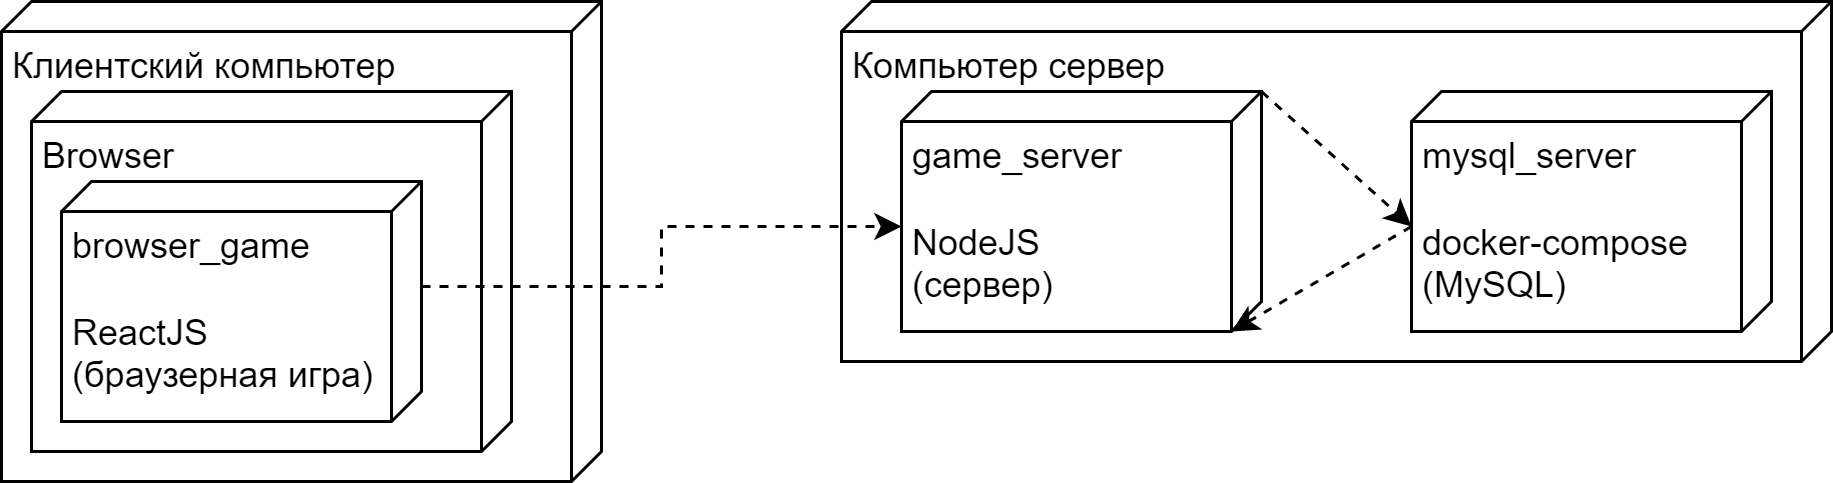
\includegraphics[width=16cm]
            {../sources/game_architecture/build/game__deployment_diagram.png}
        \caption{Диаграмма развёртывания}
        \label{fig:game__deployment_diagram}
    \end{figure}

    \newpage
    \subsection{Тестирование приложения}


    \subsubsection*{Тестирование просмотра своих карт в руках}

    \textit{Тестируемая задача}: \underline{Просмотр своих карт в руках}.
    
    \textit{Ожидаемый результат}: видны карты в руках.

    \textit{Полученный результат}:

    \textit{Вывод по тесту}:


    \subsubsection*{Тестирование добавление карты на стол}

    \textit{Тестируемая задача}: \underline{Добавление карты на стол}.
    
    \textit{Ожидаемый результат}: выбранная карта положилась на стол.

    \textit{Полученный результат}:

    \textit{Вывод по тесту}:


    \subsubsection*{Тестирование окончания боя}

    \textit{Тестируемая задача}: \underline{Окончание боя}.
    
    \textit{Ожидаемый результат}: мы пропускаем ход, а противник делает последний ход.
    
    \textit{Полученный результат}:

    \textit{Вывод по тесту}:

    \newpage

    %
    \newpage
    \addcontentsline{toc}{section}{СПИСОК ИСПОЛЬЗОВАННЫХ ИСТОЧНИКОВ}
    \section*{СПИСОК ИСПОЛЬЗОВАННЫХ ИСТОЧНИКОВ}
    \begin{enumerate}
        \item[1.] Леоненков А. В.
        Самоучитель UML 2. -- СПб.: БХВ-Петерберг, 2007. -- 576с.
        % \item[0.] HTML title tag - [Электронный ресурс]
        % Режим доступа: \url{https://www.youtube.com/watch?v=}
        % Дата~доступа:~xx.xx.2022.
    \end{enumerate}
    \newpage
\end{document}
